\section{Introduction}
\label{sec:intro}

Reasoning Large Language Models can be compressed through structured pruning, but the pruned model must recover its reasoning capabilities through fine-tuning.
The dominant assumption is that the recovery paradigm (SFT versus RLVR) determines recovery quality: \citet{selfhealing2025} demonstrate that RLVR restores pruned reasoning models to near-original accuracy, substantially outperforming SFT.
Our results suggest that this hierarchy is attributable to suboptimal pruning rather than a fundamental property of RL\@.
When pruning preserves representational diversity, the choice of recovery paradigm has minimal effect on downstream accuracy within 20--25\% fine-grained MLP sparsity on Qwen2.5-family models: at 20\% sparsity, mean $|\Delta(\text{GRPO}-\text{SFT})| {=} 0.54$\,pp across the four fine-grained criteria (max $0.61$\,pp); including dose-response variations, MBPP, and MATH-500, the maximum observed difference is $1.8$\,pp.
The pruning criterion---not the recovery paradigm---appears to be the primary determinant of post-pruning reasoning quality.
Since RL optimizes reward as a proxy for task performance, one would expect reward improvements to translate into accuracy gains---making their divergence noteworthy.

This divergence is surprising because RL and SFT impose fundamentally different demands on model representations: RL compresses incorrect paths while SFT expands correct ones~\citep{rlsqueezes2026}. Yet existing structured pruning methods for reasoning LLMs~\citep{graspprune2026,resp2025,llmpruner2023,bonsai2025} optimize for post-pruning quality without examining how the criterion shapes downstream RL recovery.
No prior work has compared multiple pruning criteria under RL or investigated whether the ``RLVR $>$ SFT'' advantage persists across pruning strategies.
We note that \citet{selfhealing2025} evaluate unstructured magnitude pruning retaining 96.5\% of dense parameters; our findings concern fine-grained structural pruning where entire channel groups are removed, and the two settings may impose different demands on RL recovery.

\begin{figure}[t]
\centering
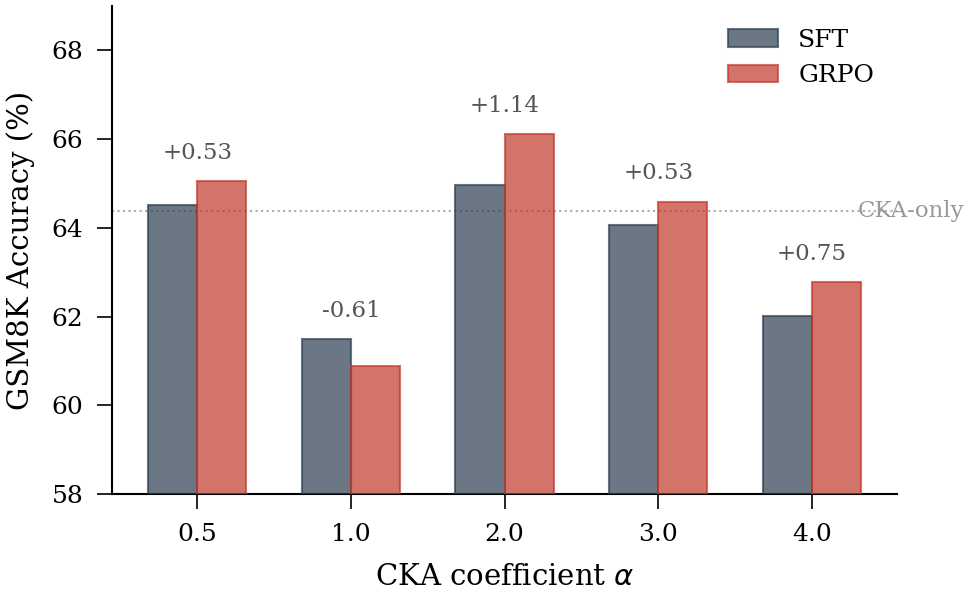
\includegraphics[width=\columnwidth]{figures/paper/fig1_dose_response.pdf}
\caption{Dose-response curve for the CKA diversity coefficient $\alpha$ at 20\% MLP channel sparsity on GSM8K ($N{=}1{,}319$). Recovery accuracy follows an inverted-U, peaking at $\alpha{=}2.0$ (66.11\%). SFT and GRPO curves nearly overlap ($|\Delta| \leq 1.14$\,pp at every point), illustrating reward-accuracy decoupling: the pruning criterion, not the recovery paradigm, determines outcome at this sparsity level.}
\label{fig:dose_response}
\end{figure}

We present a controlled comparison on DeepSeek-R1-Distill-Qwen-7B~\citep{deepseek2025r1} at 20\% MLP channel sparsity, varying the balance between gradient importance and CKA-based representational diversity~\citep{kornblith2019cka} via a coefficient $\alpha$ in the pruning score (Figure~\ref{fig:dose_response}).
The dose-response curve reveals an inverted-U: recovery peaks at $\alpha{=}2.0$ (66.11\% GRPO on GSM8K~\citep{cobbe2021gsm8k}), where importance and diversity reach optimal balance.
Under GRPO~\citep{shao2024grpo} training, four criteria produce a \textbf{recovery capacity spectrum}---a gradient in the pruned model's ability to regain reasoning through post-hoc training---ranging from active learning (CKA-only, peak reward 4.4$\times$ Standard) through stagnation (Random) to reward collapse (\rasp{} at $\alpha{=}1.0$), that tracks preserved representational diversity rather than gradient importance.
A depth pruning baseline (ShortGPT;~\citealp{shortgpt2024}) is the only method with $|\Delta| > 1$\,pp on GSM8K ($-$1.36\,pp), suggesting that pruning granularity interacts with RL trainability.

Our contributions are:
\begin{enumerate}[nosep,leftmargin=*]
    \item \textbf{Reward-accuracy decoupling.} At 20--25\% sparsity, GRPO and SFT produce near-identical accuracy across all four fine-grained criteria (mean $|\Delta| {=} 0.54$\,pp; max $1.8$\,pp including dose-response, MBPP, MATH-500). At 15\%, GRPO amplifies the CKA-guided advantage ($+$1.51\,pp), but this exception reinforces the main pattern (\S\ref{sec:decoupling}).
    \item \textbf{Recovery capacity spectrum.} We propose Recovery-Aware Structured Pruning (\rasp{}), combining gradient importance with CKA-based diversity via $\alpha$. Dose-response reveals an inverted-U peaking at $\alpha{=}2.0$ (66.11\% on GSM8K). Four criteria produce qualitatively distinct GRPO dynamics---from active learning to reward collapse---tracking preserved diversity. Preliminary evidence at 1.5B and across Qwen2.5-family models (\S\ref{sec:scoring}, \S\ref{sec:recovery_gradient}, \S\ref{sec:extended_analysis}).
\end{enumerate}

\begin{figure*}[t]
\centering
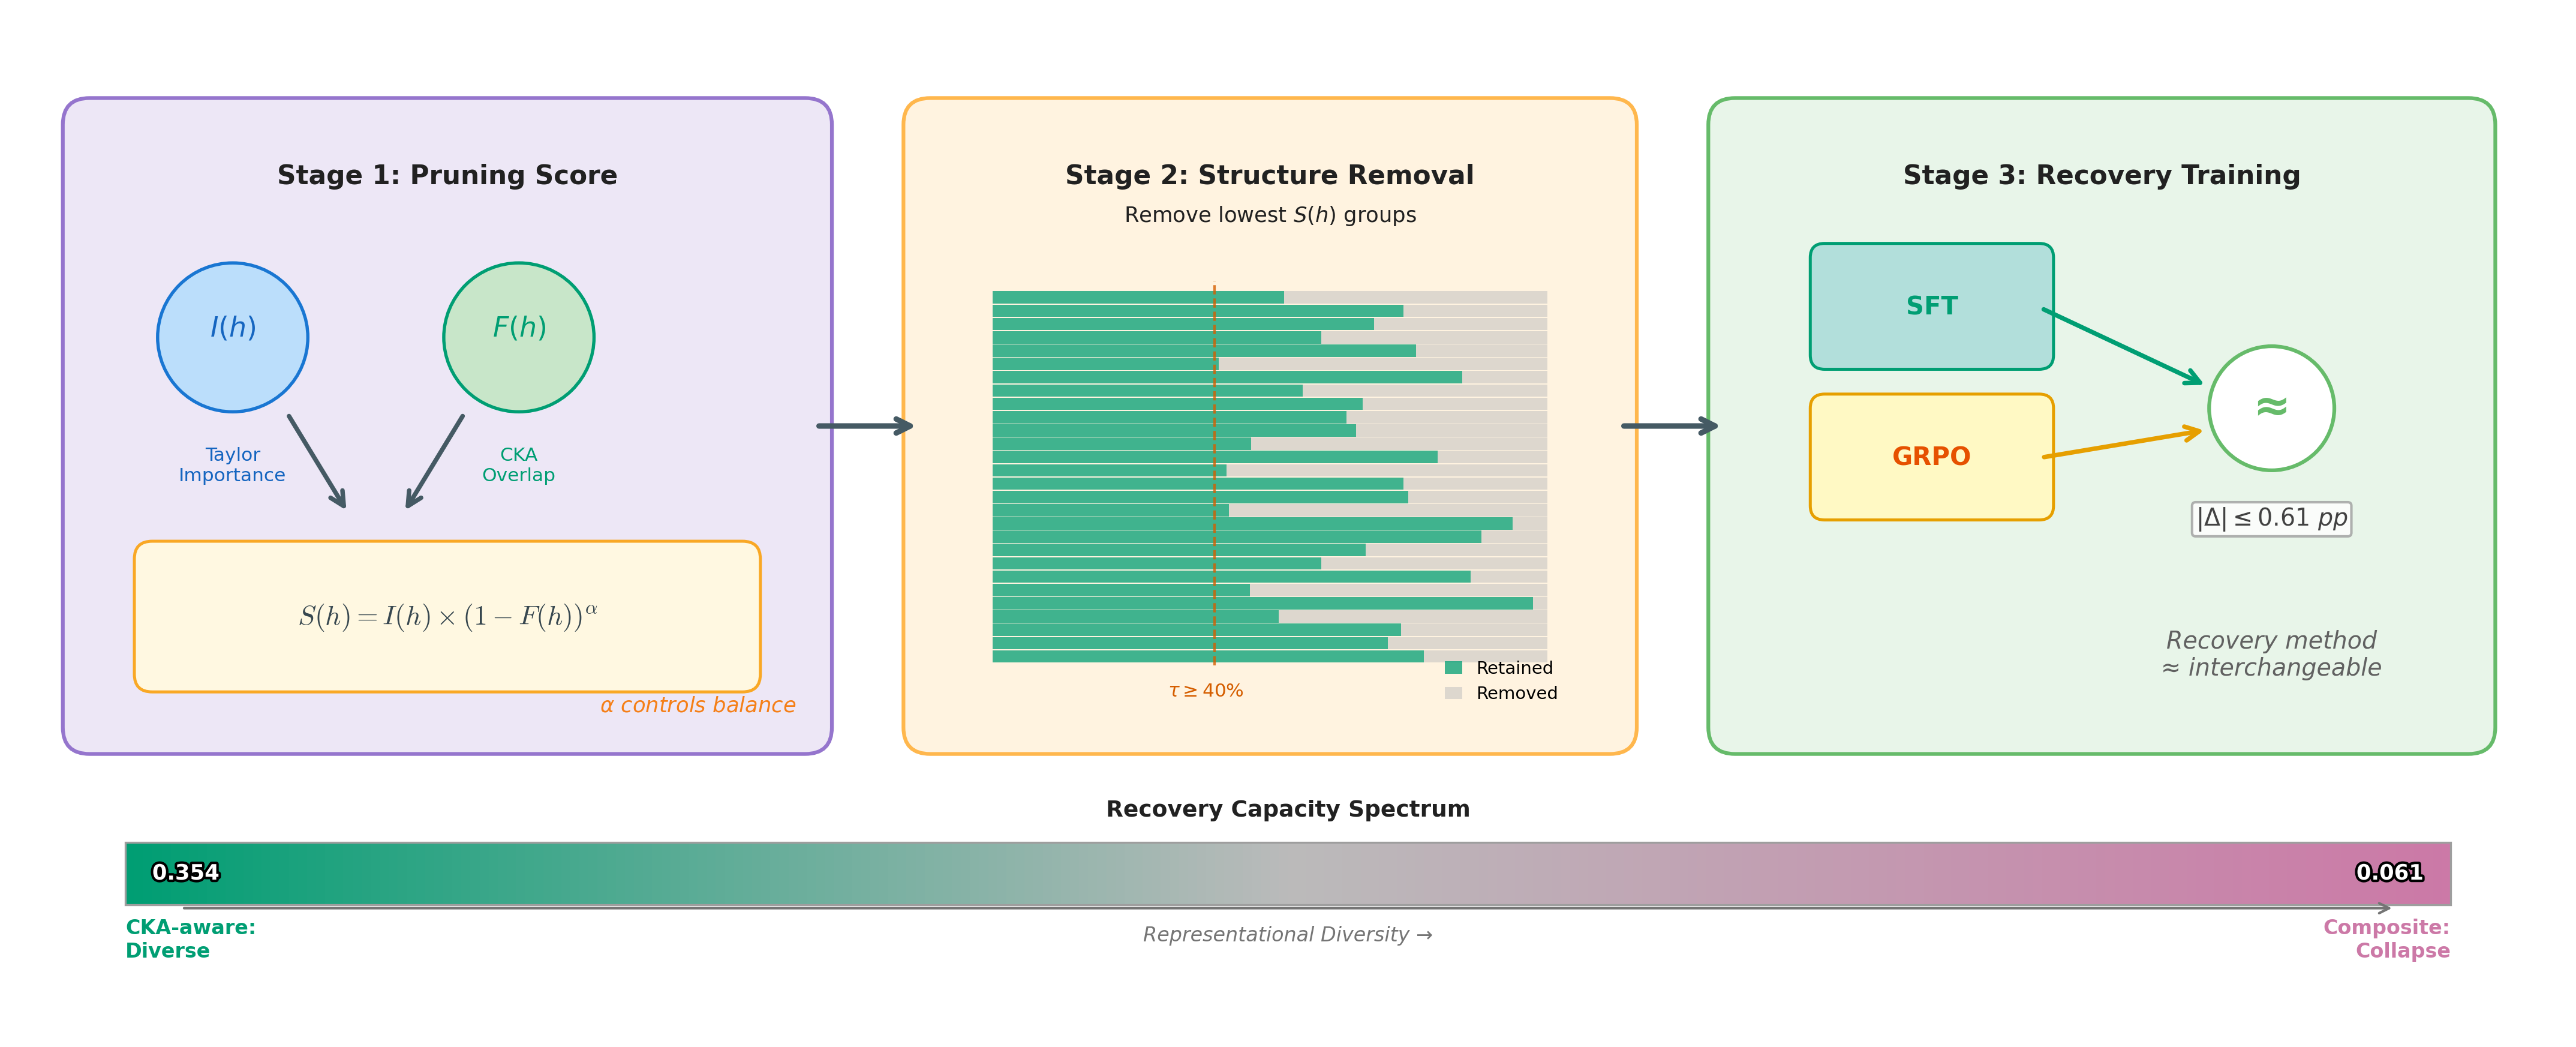
\includegraphics[width=\textwidth]{figures/paper/fig1_method_framework.pdf}
\caption{Overview of our pruning comparison framework. \textbf{Left}: structural analysis computes importance $I(h)$ and CKA-based overlap $F(h)$ scores, which four scoring criteria combine differently (Eqs.~\ref{eq:standard}--\ref{eq:cka_only}). \textbf{Center}: ranked structures are removed up to the target sparsity, subject to per-layer capacity floors. \textbf{Right}: all pruned models undergo identical two-stage recovery (SFT warmup $\to$ GRPO). \textbf{Bottom}: the resulting recovery capacity spectrum, from active learning (CKA-only) to reward collapse (\rasp{} at $\alpha{=}1.0$), tracks preserved representational diversity rather than gradient importance.}
\label{fig:method_framework}
\end{figure*}
